% Chapter Template

% Main chapter title
%\chapter[toc version]{doc version}
\chapter{Networked data streams}

% Short version of the title for the header
%\chaptermark{version for header}

% Chapter Label
% For referencing this chapter elsewhere, use \ref{ChapterTemplate}
\label{chp:networked_data_streams}

% Write text in here
% Use \subsection and \subsubsection to organize text


\begin{tcolorbox}
	\small{
		The content presented in this Chapter was partially published in or adapted from \cite{SpaMHMM, SOHMMM}.
	}
\end{tcolorbox}

\section{Motivation}
\label{sec:chp1_motivation}
A broad range of real-life settings can be well modeled by an arbitrary number of network connected entities that share and interact in the same medium and generate data streams in real-time. The streams produced by each of these entities form a set of time series with both intra- and inter-correlations between them. In neuroimaging studies, the brain can be regarded as a network: a connected system where nodes, or units, represent different specialized regions and links, or connections, represent communication pathways. From a functional perspective, communication is coded by temporal dependence between the activities of different brain areas (\citet{DeVicoFallani20130521}). Also team sports intrinsically involve fast, complex and interdependent events among a set of entities (the players), which interact as a team (\citet{Tora2017, Theagarajan2018}). The emergence of vehicular networks is also generating an ever-increasing amount of network data (\citet{Cheng2018}), where interactions between neighboring vehicles may be exploited to build more accurate and reliable learning algorithms. Thus, in all these scenarios the behavior of each individual entity is better understood if its context information (i.e.\ the behavior of the neighboring instances) is leveraged. However, the extraction of knowledge from these streams to support the decision-making process is still challenging. Moreover, conventional algorithms that assume ability to store and centralize all the data in memory at the same time are impractical for many applications (\citet{Gama2007}).

Modeling the generative process of distributed stream data is an unsupervised learning problem and, hence, a model can be learned directly from the large amounts of data that might be continuously produced or gathered at each network connected entity, without the requirement of any special human supervision or annotation. Moreover, generative models are powerful tools for a wide variety of problems that arise naturally in networked data streams, like anomaly and novelty detection, sequence forecasting, clustering, and network simulation. Hence, generative models for stream data have been developed and applied in several previous works (e.g.\ \citet{Laxman2008, Hayat2010, Hofmann2011}). However, to the best of our knowledge, this problem is seldom explored in the  distributed setting.

Given the distributed nature of network data and the high information rate that those streams could have, we argue that such generative model and/or the associated learning algorithm should ideally satisfy the following properties:
\begin{enumerate}
	\item Learning and inferring distributedly, i.e.\ each entity should be able to update its own model and perform inference on it without observing the streams or the models associated with the remaining entities.
	\item Learning online, i.e.\ in real-time and without the requirement of storing the whole dataset in memory.
	\item Leveraging contextual information by incorporating prior knowledge about similarities and dissimilarities among sets of entities.
	\item Universality, i.e.\ the model should be applicable to a wide variety of distributed stream data, of diverse nature.
\end{enumerate}
In this chapter, we present two solutions for this problem, each with its own advantages and drawbacks. Both are inspired on the concept of sparse representations, which expresses a signal/model $f$, defined over some independent variable $x$, as a linear combination of a few atoms from a prespecified and overcomplete dictionary of size $M$:
\begin{equation}
\label{sparse_coding}
f(x)=\sum_{m=1}^M s_m \phi_m(x),
\end{equation}
where $\phi_m(x)$ are the atoms and only a few of the scalars $s_m$ are non-zero, providing a sparse representation of $f(x)$.  Distributed sparse representation (\citet{Baron}) is an extension of the standard version that considers networks with $K$ nodes. At each node, the signal sensed at the same node has its sparsity property because of its intracorrelation, while, for networks with multiple nodes, signals received at different nodes also exhibit strong intercorrelation.
The intra- and inter-correlations lead to a joint sparse model. An interesting scenario in distributed sparse representation, which we exploit here, is when all signals/models share the common support but with different non-zero coefficients.

Our contributions in this chapter are summarized as follows: i) we extend an existing model based on a combination of self-organizing maps (SOM) and HMMs and evaluate it in the context of anomaly detection in Wi-Fi networks; ii) we present a novel algorithm that learns an entity-dependent model based on a mixture of shared HMMs; iii) we discuss how the two models intersect each other and, importantly, how the latter can be viewed as a particular case of a general family of generative models for distributed data.

\section{Hidden Markov Models on a Self-Organizing Map for Anomaly Detection in 802.11 Wireless Networks}
\label{sec:sohmmm}

\subsection{Introduction}
\label{sec:sohmmm_intro}
In large-scale 802.11 wireless networks, acquiring a baseline knowledge of the entire infrastructure is not straightforward. Owing to the time-varying and physically distributed nature of these networks, learning the usage characteristics of access points (APs), users, and locations becomes more and more challenging. The wireless-channel conditions evolve over time, as does the usage behavior of the wireless users in different parts of the network. Thus, the wireless users are likely to suffer from many types of connectivity and performance problems, e.g., interference, intermittent connections, or authentication failures. To constantly ensure that wireless users have reliable connections, network managers require tools and techniques to monitor the network, identify the problems, and resolve them efficiently.

Naive approaches, e.g., using a single HMM common to all APs, lose the flexibility to adapt to the specificities of each AP, while using one HMM per AP, trained independently from the others, fails to leverage the relations between observations of neighboring APs. HMM initialized with universal background model (HMM-UBM) \cite{Anisa2017} is an improvement in the right direction; however, the relations between APs are only used in the initial phase, where one trains the UBM to then initialize the individual HMM models for each AP. Thereafter, the individual HMMs evolve independently, only benefiting from the AP's own data. Although this is a very sensible approach in the biometrics and speech-modeling fields, where HMM-UBM has been used to robustly train user-specific models, in our setting, it fails to properly explore the dependencies between data from APs with similar behavior. 

In the current work, we focus on the actual proximity of APs as a determining factor in connectivity and performance problems. Anomalous cases, e.g., across-AP-vicinity interference, AP overloads, or AP shutdown/halt could eventually affect the usage behavior of the other APs in the neighborhood. To consider such behavioral changes in the local area and their respective influences, we employ the synergistic approach of self-organizing hidden Markov model map (SOHMMM) to exploit the semantic connectivity between adjacent HMMs.

The self-organizing map is an artificial neural network that defines a nonlinear transformation from the input space to the set of nodes in the output space \cite{Ref8}. Each node or neuron in the SOM is associated with a model of the input space. Through an unsupervised-learning process, the models are tuned and organized in a lattice topology according to the input patterns. In SOHMMM, each neuron is literally associated with an HMM.  

The training processes of the SOM and HMM sub-units are, in most cases, disjoint and conducted independently. There are two main approaches regarding these hybrid techniques. The first approach considers the SOM as a front-end processor (e.g., vector quantization, preprocessing, feature extraction); HMMs are then used in the higher processing stages \cite{Somervuo2000,Kurimo1996,Morimoto2016}. The second approach places the SOM on top of the HMM \cite{Ferles2013,Ferles2013b,Lebbah2015}.   

In SOHMMM, the SOM unsupervised-learning approach is well combined with the HMM dynamic-programming technique. The structure of both corresponding components is unified in an integrated super-model. The presented online gradient-descent unsupervised-learning algorithm is inspired by the SOHMMM algorithm previously proposed in \cite{Ferles2013} and originated in \cite{Baldi1994}. We extend the model to fit the requirements of our anomaly-detection problem and improve the presented algorithm in \cite{Ferles2013} for multivariate Gaussian emissions\footnote{In \cite{Ferles2013}, only the discrete-observation setting is addressed.}.

\subsection{Related work}
A number of studies in the literature have integrated the SOM and HMM in different manners. In \citet{Gen2012}, the spherical self-organizing map (S-SOM) is proposed, which uses HMM models as neurons (S-HMM-SOM) to classify the time-series data. Despite our work, the HMM models in \citet{Gen2012} are discrete and the author applied the  Baum-Welch algorithm for updating the model parameters. In \citet{Yamaguchi2010}, the authors extended the self-organizing mixture models for multivariate time-series, assuming that the time-series are generated by HMMs. This model, which is called a self-organizing hidden Markov model (SOHMM), uses constrained expectation maximization (EM) for HMM parameter estimation. The self-organization in this work is used for meteorological-state visualization. 

In another direction of work in \citet{Caridakis2010}, a SOMM-based architecture is presented for hand-gesture recognition. The approach involves a combination of SOMs and Markov models for gesture-trajectory classification. In this work, the neurons on the SOM map correspond to the states of the Markov models. In \citet{Jaziri2011}, the combination of the SOM and HMM (SOS-HMM: self-organizing structure of HMM) automatically extracts the structure of an HMM without any prior knowledge of the application domain. In this model, the macro-HMM is represented as a graph of macro-states, where each state represents a micro-HMM. In summary, each neuron in the SOM-HMM collaborative architecture is either an HMM by itself or a hidden state. In our work, each particular neuron on the SOM lattice is associated with an HMM. 

In \citet{Lebbah2015}, a probabilistic self-organizing map called PrSOMS is presented for the clustering and visualization of dependent and non-identically distributed data. In this model, the SOM learning paradigm to produce topology-preserving maps is combined with the probabilistic-learning scheme of the HMM. The SOM is considered to be a grid, forming a discrete topology in which each cell represents a state; the parameters of the model are estimated by maximizing the likelihood of the sequential data set. In another direction of work in \citet{Morimoto2016}, the effects of meteorological factors on the occurrence of strokes are investigated. The authors used the SOM to obtain weather patterns that would serve as states of the HMMs. They showed that HMMs with states given by the SOM are useful for describing a background process of stroke incidence. This approach considers the SOM as a front-end processor.

In \citet{Ferles2008,Ferles2013,Ferles2017}, the fusion and synergy of SOMs and HMMs are employed in biological-molecule studies to meet the increasing requirements imposed by the properties of deoxyribonucleic acid (DNA), ribonucleic acid (RNA), and protein chain molecules. The authors proposed a stochastic unsupervised-learning algorithm based on the integration of the SOM and HMM principles, called self-organizing hidden Markov model map (SOHMMM). The SOHMMM characteristics and capabilities are demonstrated through two series of experiments, based on artificial sequence data and splice-junction gene sequences. However, in these papers, only the discrete-observation setting is addressed. Here, we extend the algorithm for multivariate Gaussian in order to fit the requirements of our anomaly-detection project.

Incremental learning of HMM parameters is the core function of the SOHMMM algorithm, which is based on a stochastic gradient-descent technique. The incremental learning of new data sequences allows HMM parameters to adapt as new data become available, without having to retrain from the start on all the accumulated training data. Various techniques in the literature address this topic. These techniques are classified according to the objective function, optimization technique, and target application, involving the block-wise and symbol-wise learning of parameters. The authors in \citet{Khreich2012} presented a comprehensive survey of techniques that are suitable for the incremental learning of HMM parameters, among which, the stochastic gradient-descent technique of the SOHMMM is referred to as one of the numerical-optimization methods.

Additionally, few efforts exist in the literature that exploit the SOM and HMM for anomaly-detection purposes (\citet{Cho2002,Wang2006}). In \citet{Cho2002}, the authors presented an intrusion-detection system in which the SOM determines the optimal measures of audit data and reduces them to an appropriate size for efficient modeling by the HMM. Two types of HMM are utilized: a single model for all the users and individual models for each user. In another relevant work by \citet{Wang2006}, the HMM and the SOM are investigated separately as intrusion-detection techniques. The testing results show that the HMM method using the events' transition property outperformed the SOM using the events' frequency property. Regarding the same subject of intrusion detection, the SOM and HMM have a collaborating connection in \citet{Cho2002} and competitive roles in \citet{Wang2006}.

In this work, we intend to benefit from the collaboration of these two techniques (SOM and HMM), as proposed by \citet{Ferles2008}, to extend previous anomaly-detection frameworks applying only HMM (\citet{Anisa2014,Anisa2017,Anisa2019}).

\subsection{The Self-Organizing Hidden Markov Model Map for Discrete Observations}
\label{sec:sohmmm_background}

We start by reviewing SOHMMM as initially formulated by \citet{Ferles2008}. This model defines a mapping between an observed sequence $\rvx \triangleq \left(\rx^{(1)}, \dots, \rx^{(t)} \right)$ and a two-dimensional lattice of HMMs, which constitute its nodes. Each observation is assumed to be discrete, so $\rvx^{(\tau)} \in \{1,\dots,o\}$, being $o$ the size of the dictionary of observations. The topology of a 2-D lattice of $m$ HMMs is defined by a function $\vr: \{1, \dots, m\} \mapsto \mathbb{R}^2$, mapping the indices of the $m$ nodes to the respective coordinates in the plane. Given the lattice topology, a neighborhood function $v: \{1, \dots, m\}^2 \mapsto [0, \infty)$ can be defined mapping two nodes in the lattice to a scalar representing how close the two nodes are. In SOHMMM, $v$ is a Gaussian kernel:
\begin{equation}
\label{eq:sohmmm_distance}
v(z,z') \triangleq \exp\left(-\lambda||\vr(z)-\vr(z')||^{2}\right),
\end{equation}
where $\lambda > 0$ is a hyperparameter controlling the rate of the decay.
Following the idea of SOMs, the SOHMMM algorithm aims to minimize an \emph{energy function}, defined below:
\begin{equation}
\label{eq:sohmmm_energy}
E(\vx; \Theta) \triangleq -\sum_{\rz} p(\vx \mid \rz, \Theta)v(\rz, z^*),
\end{equation}
where $\theta$ summarizes all parameters of the HMMs, $\rz$ indexes the $m$ HMMs in the lattice, and $p(\rvx \mid \rz)$ is the marginal distribution of observations of a standard HMM:
\begin{equation}
\label{eq:sohmmm_hmm}
p(\rvx \mid \rz) = \sum_{\rvh} p(\rh^{(0)} \mid \rz) \prod_{\tau=1}^t p(\rh^{(\tau)} \mid \rh^{(\tau-1)},\rz) p(\rx^{(\tau)} \mid \rh^{(\tau)},\rz),
\end{equation}
where $\rvh = \left(\rh^{(0)},\dots,\rh^{(t)}\right)$ is the sequence of hidden states of the HMM and $\rh^{(\tau)} \in \{1, \dots, s\}$, being $s$ the number of hidden states. Finally, $z^*$ corresponds to the index of the \emph{winner node} for the observation $\vx$:
\begin{equation}
\label{eq:sohmmm_winner}
z^* \triangleq \argmax_{z' \in \{1,\dots,m\}} \sum_{\rz} p(\vx \mid \rz, \Theta)v(\rz, z').
\end{equation}

The set $\Theta$ consists of the following parameters:
\begin{itemize}
	\item the $s$-dimensional initial state probabilities, $\vpi^{(z)}$, where $\evpi_h^{(z)} \triangleq p(\rh^{(0)}=h \mid \rz=z)$, for $h \in \{1,\dots,s\}$ and $z \in \{1,\dots,m\}$;
	\item the $s \times s$ state transition matrices, $\mA^{(z)}$, where $\emA^{(z)}_{h,h'} \triangleq p(\rh^{(t)}=h' \mid \rh^{(t-1)}=h, \rz=z)$, for $h,h' \in \{1,\dots,s\}$ and $z \in \{1,\dots,m\}$;
	\item the $s \times o$ emission probability matrices, $\mB^{(z)}$, where $\emB^{(z)}_{h,x} \triangleq p(\rx^{(\tau)}=x \mid \rh^{(\tau)}=h, \rz=z)$, for $h \in \{1,\dots,s\}$, $x \in \{1,\dots,o\}$, and $z \in \{1,\dots,m\}$.
\end{itemize}
Thus, $\Theta \triangleq \{(\vpi^{(z)}, \mA^{(z)}, \mB^{(z)})\}_{z=1}^m$, where each triplet $(\vpi^{(z)}, \mA^{(z)}, \mB^{(z)})$ completely defines one HMM in the lattice. The SOHMMM online learning algorithm corresponds to stochastic gradient descent over the energy function~\plaineqref{eq:sohmmm_energy}. Constrained optimization is avoided by reparametrizing the model using softmax functions, so that standard, unconstrained stochastic gradient descent can be performed over the new parameters $\vu^{(z)}$, $\mW^{(z)}$, and $\mR^{(z)}$:
\begin{equation}
\evpi_h^{(z)} = \frac{\exp(\evu_h^{(z)})}{\sum_{h'=1}^{s}\exp(\evu_{h'}^{(z)})}, \quad
\emA^{(z)}_{h,h'} = \frac{\exp(\emW^{(z)}_{h,h'})}{\sum_{h''=1}^{s} \exp(\emW^{(z)}_{h,h''})}, \quad
\emB^{(z)}_{h,x} = \frac{\exp(\emR^{(z)}_{h,x})}{\sum_{x'=1}^{o} \exp(\emR^{(z)}_{h,x'})}.
\end{equation}
The full algorithm, comprising the update equations for each parameter, is presented in \Algref{alg:sohmmm_discrete} and its derivation can be found in \citet{Ferles2008}.

\begin{algorithm}
	\caption{SOHMMM Learning Algorithm for Discrete Observations \cite{Ferles2008}}
	\label{alg:sohmmm_discrete}
	
	\begin{algorithmic}[1]
		\State \textbf{Inputs:} the lattice $r$ with $m$ nodes, the hyperparameter $\lambda$ of the neighborhood function $v$, the set of initial parameters $\Theta^{(0)}$, the learning rate $\eta$, and the number of training iterations \texttt{trainIter}.
		\vspace{0.3cm}
		\For{$i = 1, \dots,$\texttt{trainIter}} 
		\vspace{0.3cm}
		\State Observe $\rvx = \vx$, with length $t$.
		\vspace{0.3cm}
		\For{$z = 1, \dots, m$} $\quad$(Forward-Backward algorithm)
		\vspace{0.3cm}
		\State $ \alpha_1^{(z)}(h) \coloneqq \pi_{h}^{(z)}\emB^{(z)}_{h,x^{(1)}}, \quad h = 1, \dots, s$;
		\vspace{0.3cm}
		\State $ \alpha_{\tau+1}^{(z)}(h) \coloneqq \emB^{(z)}_{h,x^{(\tau+1)}} \sum_{h'=1}^{s}\alpha_{\tau+1}^{(z)}(h')\emA^{(z)}_{h',h}, \quad \tau = 1, \dots, t-1, \quad h = 1, \dots, s;$
		\vspace{0.3cm}
		\State $ \beta_{t}^{(z)}(h) \coloneqq 1, \quad h = 1, \dots, s;$
		\vspace{0.3cm}
		\State $ \beta_{\tau}^{(z)}(h) \coloneqq \sum_{h'=1}^{s}\emA^{(z)}_{h,h'}\emB^{(z)}_{h,x^{(\tau+1)}}\beta_{\tau+1}^{(z)}(h'), \quad \tau = t-1, \dots,  1, \quad h = 1, \dots, s. $
		\vspace{0.3cm}
		\EndFor
		\vspace{0.3cm}
		\State $z^* \coloneqq  \argmax_{z' \in \{1,\dots,m\}} \sum_{z=1}^m p(\vx \mid z, \Theta^{(i-1)})v(z, z')$.
		\vspace{0.3cm}
		\For{$z = 1, \dots, m$}
		\vspace{0.3cm}
		\State $ \evu_h^{(z)} \coloneqq \evu_h^{(z)} + \eta  \evpi_h^{(z)} \left[ \emB^{(z)}_{h,x^{(1)}} \beta_{1}^{(z)}(h) - p(\vx \mid z, \Theta^{(i-1)}) \right], \quad h = 1, \dots, s;$
		\vspace{0.3cm}
		\State $ \emW^{(z)}_{h,h'} \coloneqq  \emW^{(z)}_{h,h'} + \eta v(z,z^*) \emA^{(z)}_{h',h}\sum_{\tau=1}^{t-1}\left[\alpha_{\tau}^{(z)}(h) \emB^{(z)}_{h,x^{(\tau+1)}}\beta_{\tau+1}^{(z)}(h') - \alpha_{\tau}^{(z)}(h)\beta_{\tau}^{(z)}(h) \right], \quad h,h' = 1, \dots, s; $
		\vspace{0.3cm}
		\State $ \emR^{(z)}_{h,x'} \coloneqq \emR^{(z)}_{h,x'} + \eta v(z,z^*) \sum_{\tau=1}^{t}\left[\1_{x^{(\tau)}=x'}\alpha_{\tau}^{(z)}(h)\beta_{\tau}(h) - \emB^{(z)}_{h,x'}\alpha_{\tau}^{(z)}(h)\beta_{\tau}^{(z)}(h) \right], \quad h = 1, \dots, s, \quad x' = 1,\dots,o;$
		\vspace{0.3cm}
		\State $\evpi_h^{(z)} \coloneqq \exp(\evu_h^{(z)}) \big/ \sum_{h'=1}^{s}\exp(\evu_{h'}^{(z)}), \quad h = 1, \dots, s;$
		\vspace{0.3cm}
		\State $ \emA^{(z)}_{h,h'} \coloneqq \exp(\emW^{(z)}_{h,h'}) \big/ \sum_{h''=1}^{s} \exp(\emW^{(z)}_{h,h''}), \quad h,h' = 1, \dots, s;$
		\vspace{0.3cm}
		\State $\emB^{(z)}_{h,x'} \coloneqq \exp(\emR^{(z)}_{h,x'}) \big/ \sum_{x''=1}^{o} \exp(\emR^{(z)}_{h,x''}), \quad h = 1, \dots, s, \quad x' = 1,\dots,o.$
		\vspace{0.3cm}
		\EndFor
		\vspace{0.3cm}
		\State $\Theta^{(i)} \coloneqq \lbrace (\vu^{(z)}, \mW^{(z)}, \mR^{(z)}) \rbrace_{z=1}^m$.
		\vspace{0.3cm}
		\EndFor
		
	\end{algorithmic}
\end{algorithm}

\subsection{Extending SOHMMM to Gaussian Observations}
\label{sec:sohmmm_gaussian}

For the purpose of modeling AP usage data, we should consider a slightly different setting where each observation $\rvx^{(\tau)}$ takes values on the $d$-dimensional plane $\sR^d$, rather than being drawn from a discrete and finite set. Hence, now, sequences $\rmX \triangleq \left(\rvx^{(1)}, \dots, \rvx^{(t)} \right)$ take values on $\sR^{d \times t}$. A sensible option, which may be useful in a broad range of applications, is considering the case of multivariate Gaussian emissions, i.e. $\rvx^{(\tau)} \mid (\rh^{(\tau)}, \rz) \sim \mathcal{N}\left(\vx; \vmu^{(z)}_h, \mSigma^{(z)}_h\right)$, where $\vmu^{(z)}_h \in \sR^d$ is the mean and $\mSigma^{(z)}_h \in \sR^{d \times d}$ is the covariance of the Gaussian component corresponding to state $h$ in the lattice node $z$. These means and covariances replace the emission probability matrices $\mB^{(z)}$ defined for the case of discrete observations.

We shall now derive the necessary readjustments in \Algref{alg:sohmmm_discrete}. Let us denote by $\vx$ the observation at a given time $\tau$ (i.e., $\rvx^{(\tau)}=\vx$) and consider the corresponding state $\rh^{(\tau)}$ and the node $\rz$ as fixed at $h$ and $z$, respectively. Thus, we use the notation $p(\vx \mid h, z)$ as a short for $p(\rvx^{(\tau)}=\vx \mid \rh^{(\tau)}=h, \rz=z)$. We have:
\begin{align}
\frac{\partial p(\mX \mid z)}{\partial p(\vx \mid h, z)} &= \frac{\partial}{\partial p(\vx \mid h, z)} \left[\sum_{\rvh} p(\mX, \rvh \mid z)  \right] \nonumber\\
&= \frac{\partial}{\partial p(\vx \mid h, z)} \left[\sum_{\rvh} p(\rh^{(0)} \mid \rz) \prod_{\tau'=1}^t p(\rh^{(\tau')} \mid \rh^{(\tau'-1)},\rz) p(\rvx^{(\tau')} \mid \rh^{(\tau')},\rz)\right] \nonumber\\
&= \frac{1}{p(\vx \mid h, z)} \sum_{\rvh:\, \rh^{(\tau)}=h} p(\mX, \rvh \mid z) \nonumber\\
&= \frac{p(\mX, h \mid z)}{p(\vx \mid h, z)} \nonumber\\
&= \frac{\alpha_{\tau}^{(z)}(h) \beta_{\tau}^{(z)}(h)}{p(\vx \mid h, z)}.
\end{align}
Note that, for discrete observations, $p(x \mid h, z) = \emB^{(z)}_{h,x}$. However, when we consider the multivariate Gaussian case,
\begin{align}
p(\vx \mid h, z) &= \mathcal{N}\left(\vx; \vmu^{(z)}_h, \mSigma^{(z)}_h\right) \nonumber\\
&= \frac{1}{\sqrt{(2\pi)^d \mathrm{det}(\mSigma^{(z)}_h)}} \exp \left(-\frac{1}{2} {(\vx - \vmu^{(z)}_h)}\transp {\mSigma^{(z)}_h}^{-1} (\vx - \vmu^{(z)}_h)\right),
\end{align}
where the covariance matrix $\mSigma^{(z)}_h$ must be positive definite. This constraint can be easily guaranteed by reparametrizing it as $\mSigma^{(z)}_h = \mS^{(z)}_h {\mS^{(z)}_h}\transp$, where $\mS^{(z)}_h \in \sR^{d \times d}$ is constraint-free. The required gradients are:
\begin{align}
&\nabla_{\vmu^{(z)}_h} p(\vx \mid h, z) = p(\vx \mid h, z) (\mS \mS\transp)^{-1} (\vx - \vmu), \\
&\nabla_{\mS^{(z)}_h} p(\vx \mid h, z) = p(\vx \mid h, z) \mS^{-1} \left[ (\vx - \vmu) (\vx - \vmu)\transp (\mS \mS \transp)^{-1} - I_d\right],
\end{align}
where we have abbreviated $\vmu^{(z)}_h$ as $\vmu$ and $\mS^{(z)}_h$ as $\mS$ to alleviate the notation. Now, by the chain rule,
\begin{align}
\nabla_{\vmu^{(z)}_h} p(\mX \mid z) &= \sum_{\tau=1}^t \frac{\partial p(\mX \mid z)}{\partial p(\vx^{(\tau)} \mid h, z)} \nabla_{\vmu^{(z)}_h} p(\vx^{(\tau)} \mid h, z) \nonumber\\
&= \sum_{\tau=1}^t \frac{\alpha_{\tau}^{(z)}(h) \beta_{\tau}^{(z)}(h)}{p(\vx^{(\tau)} \mid h, z)} \nabla_{\vmu^{(z)}_h} p(\vx^{(\tau)} \mid h, z) \nonumber\\
&= \sum_{\tau=1}^t \alpha_{\tau}^{(z)}(h) \beta_{\tau}^{(z)}(h) (\mS \mS \transp)^{-1} (\vx^{(\tau)} - \vmu), \\
\nabla_{\mS^{(z)}_h} p(\mX \mid z) &= \sum_{\tau=1}^t \alpha_{\tau}^{(z)}(h) \beta_{\tau}^{(z)}(h) \mS^{-1} \left[ (\vx^{(\tau)} - \vmu) (\vx^{(\tau)} - \vmu)\transp (\mS \mS \transp)^{-1} - I_d\right].
\end{align}
Finally, by applying the chain rule once again, we get the desired gradients of the energy function $E$ with respect to $\vmu^{(z)}_h$ and $\mS^{(z)}_h$:
\begin{align}
\nabla_{\vmu^{(z)}_h} E(\mX) &= \frac{\partial E}{\partial p(\mX \mid z)} \nabla_{\vmu^{(z)}_h} p(\mX \mid z) \nonumber\\
&= -v(z, z^*) \nabla_{\vmu^{(z)}_h} p(\mX \mid z) \nonumber\\
&= -v(z, z^*) \sum_{\tau=1}^t \alpha_{\tau}^{(z)}(h) \beta_{\tau}^{(z)}(h) (\mS \mS \transp)^{-1} (\vx^{(\tau)} - \vmu), \label{eq:sohmmm_grad_mu}\\
\nabla_{\mS^{(z)}_h} E(\mX) &= -v(z, z^*) \sum_{\tau=1}^t \alpha_{\tau}^{(z)}(h) \beta_{\tau}^{(z)}(h) \mS^{-1} \left[ (\vx^{(\tau)} - \vmu) (\vx^{(\tau)} - \vmu)\transp (\mS \mS \transp)^{-1} - I_d\right]. \label{eq:sohmmm_grad_s}
\end{align}
Given \twoeqrefs{eq:sohmmm_grad_mu}{eq:sohmmm_grad_s}, it is straightforward to adapt \Algref{alg:sohmmm_discrete} to our setting. For completeness, the full algorithm is provided in \Algref{alg:sohmmm_gaussian}.

\begin{algorithm}
	\caption{SOHMMM Learning Algorithm for Gaussian Observations}
	\label{alg:sohmmm_gaussian}
	
	\begin{algorithmic}[1]
		\State \textbf{Inputs:} Same as in \Algref{alg:sohmmm_discrete}.
		\vspace{0.3cm}
		\For{$i = 1, \dots,$\texttt{trainIter}} 
		\vspace{0.3cm}
		\State Observe $\rmX = \mX$, with length $t$.
		\vspace{0.3cm}
		\State Proceed as in lines 4--8 of \Algref{alg:sohmmm_discrete}, replacing all occurrences of $\emB^{(z)}_{h,x^{(\tau)}}$ with $\mathcal{N}\left(\vx^{(\tau)}; \vmu^{(z)}_h, \mS^{(z)}_h {\mS^{(z)}_h}\transp\right)$.
		\vspace{0.3cm}
		\State $z^* \coloneqq  \argmax_{z' \in \{1,\dots,m\}} \sum_{z=1}^m p(\mX \mid z, \Theta^{(i-1)})v(z, z')$.
		\vspace{0.3cm}
		\For{$z = 1, \dots, m$}
		\vspace{0.3cm}
		\State Proceed as in lines 12 and 13 of \Algref{alg:sohmmm_discrete}, replacing all occurrences of $\emB^{(z)}_{h,x^{(\tau)}}$ with $\mathcal{N}\left(\vx^{(\tau)}; \vmu^{(z)}_h, \mS^{(z)}_h {\mS^{(z)}_h}\transp\right)$ and all occurences of $\vx$ with $\mX$;
		\vspace{0.3cm}
		\State $\vmu^{(z)}_h \coloneqq \vmu^{(z)}_h + \eta v(z, z^*) \sum_{\tau=1}^t \alpha_{\tau}^{(z)}(h) \beta_{\tau}^{(z)}(h) (\mS^{(z)}_h {\mS^{(z)}_h} \transp)^{-1} (\vx^{(\tau)} - \vmu^{(z)}_h), \quad h = 1, \dots, s;$
		\vspace{0.3cm}
		\State $\begin{aligned}
			\mS^{(z)}_h \coloneqq \mS^{(z)}_h + \eta &v(z, z^*) \sum_{\tau=1}^t \alpha_{\tau}^{(z)}(h) \beta_{\tau}^{(z)}(h) {\mS^{(z)}_h}^{-1} \cdot \\
			&\cdot \left[ (\vx^{(\tau)} - \vmu^{(z)}_h) (\vx^{(\tau)} - \vmu^{(z)}_h)\transp (\mS^{(z)}_h {\mS^{(z)}_h} \transp)^{-1} - I_d\right], \quad h = 1, \dots, s;
			\end{aligned}$
		\vspace{0.3cm}
		\State Proceed as in lines 15 and 16 of \Algref{alg:sohmmm_discrete}.
		\vspace{0.3cm}
		\EndFor
		\vspace{0.3cm}
		\State $\Theta^{(i)} \coloneqq \lbrace (\vu^{(z)}, \mW^{(z)}, (\vmu^{(z)}_h, \mS^{(z)}_h)_{h=1}^s) \rbrace_{z=1}^m$.
		\vspace{0.3cm}
		\EndFor
		
	\end{algorithmic}
\end{algorithm}

\subsection{Experiments}
\label{sec:sohmmm_experiments}
In this section, we consider two types of experiments to analyze the capabilities of the SOHMMM algorithm for nonlinear projection and unsupervised clustering. We first validated the accuracy and convergence of the SOHMMM using \textit{synthetic data}, and then explored its significance and efficiency in anomaly detection using \textit{wireless simulation data}.

\subsubsection{Synthetic Data}
\label{sec:sohmmm_experiment_synth}

In this experiment, we generate observations from two reference HMMs, with one-third of the observations coming from one of the models, and the remaining two-thirds from the other reference model. Then, we train a SOHMMM with six nodes, randomly initialized, with the data from the reference models. It is expected that the SOHMMM nodes would converge to the reference models, with the majority of nodes grouping around the dominant reference model. The SOHMMM nodes (HMMs initialized randomly) are organized in a $2 \times 3$ rectangular lattice, as displayed in \Figref{fig:sohmmm_lattice}. This figure shows the positions and connections of the HMMs. The Euclidean distance between adjacent HMMs is set to $1$ and the other distances are computed accordingly. For example, the distance between \textit{hmm0} and \textit{hmm4} is $2$, and between \textit{hmm0} and \textit{hmm3} is $\sqrt{2}$.

\begin{figure}[h]
	\centering
	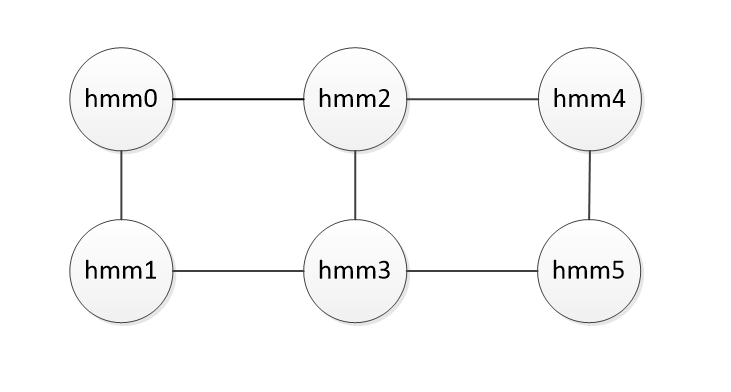
\includegraphics[scale=0.65]{ChapterTwo/lattice-rect.png}
	\caption{$2 \times 3$ rectangular lattice.}
	\label{fig:sohmmm_lattice}      
\end{figure}

In order to perform this experiment, we need a quantitative measurement of (dis)similarity between two HMMs, so that we can evaluate how close each HMM in the lattice is from the each of the two reference HMMs. It is known that two HMMs representing the same marginal distribution of observations may be parametrized by different parameters (\citet{Rabiner1989}), so the dissimilarity should not be computed in parameter space. An alternative to compare two HMMs $z$ and $z'$, proposed by \citet{Juang1985}, is the following divergence function:
\begin{equation}
D(z, z') = \frac{1}{t}\left[\log p(\mX \mid z) - \log p(\mX \mid z')\right],
\label{eq:hmm_div}
\end{equation}
where $\mX$ has length $t$ and is sampled from $p(\rmX \mid z)$. \Eqref{eq:hmm_div} is a Monte Carlo approximation of the Kullback-Leibler divergence between two HMMs \cite{Ref31} and therefore measures how well model $z'$ matches observations generated by model $z$, relative to how well model $z$ matches observations generated by itself. Since this relationship is asymmetric, we use the following symmetrized version instead:
\begin{equation}
D_{s}(z,z') = \frac{D(z,z')+D(z',z)}{2}.
\label{eq:hmm_div_sym}
\end{equation}
\Figref{fig:sohmmm_distances} demonstrates the initial and final distances between the random HMMs and the reference HMMs, upon applying the SOHMMM algorithm. The training set contains 60 observation sequences from the two reference HMMs (the \textit{ref0} model generates 40 observation sequences and \textit{ref1} generates 20). We trained the random HMMs with these observation sequences. 
Our main goal in analyzing the aforementioned distance is to examine how the observation sequences influence the random HMMs and whether they maintain their proximity while moving in different directions. Measuring this distance will indicate whether the random HMMs converge to a specific reference HMM.

\begin{figure}[h]
	\centering
	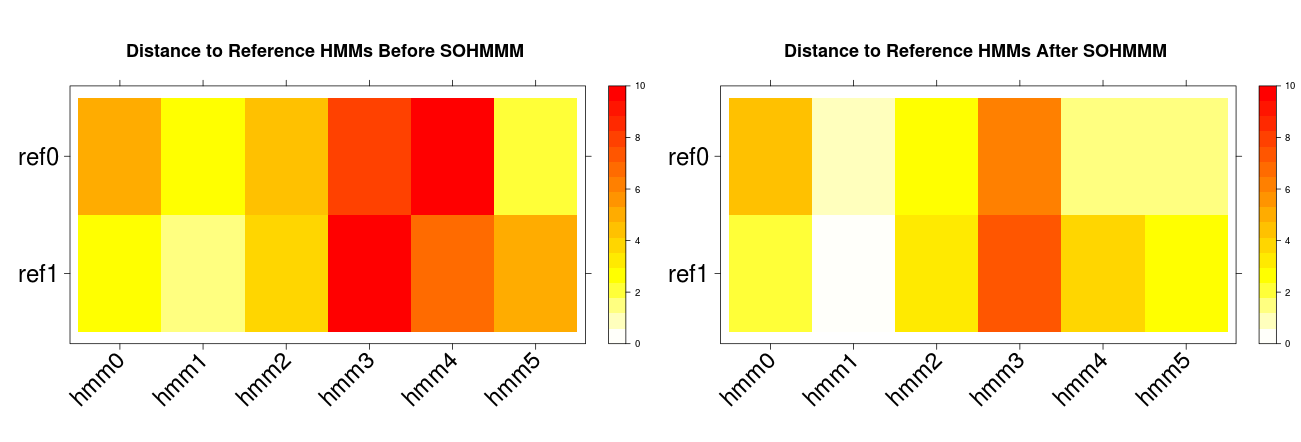
\includegraphics[scale=0.25]{ChapterTwo/hmm_ref.png}
	\caption{Monte Carlo approximation of the Kullback-Leibler divergence between the random and reference HMMs before and after applying the SOHMMM algorithm.}
	\label{fig:sohmmm_distances}      
\end{figure}

As the heatmap plots of \Figref{fig:sohmmm_distances} show, \textit{hmm4} is initially assigned to the \textit{ref1} cluster, as there is a shorter distance between these two models. After applying the algorithm, \textit{hmm4} becomes closer to \textit{ref0}. As another example, \textit{hmm3} is closer to \textit{ref0}, before and after applying the algorithm; however, the overall distance to the reference models decreases and \textit{hmm3} moves closer to both of them while maintaining its relative distance to the references. 

The minimum distance between a given random HMM and the reference HMMs defines the cluster that the HMM belongs to. In this experiment, the random HMMs belong to the $(ref1,ref1,ref1,ref0,ref1,ref0)$ and $(ref1,ref1,ref0,ref0,ref0,ref0)$ clusters, before and after applying the algorithm, respectively. The later clusters show that $\{hmm2,hmm3,hmm4\-,hmm5\}$ belong to the $ref0$ cluster, the dominant reference models; $\{hmm0,hmm1\}$ are assigned to the $ref1$ cluster, the reference model generating less data. Having analyzed the Euclidean distances of the HMM nodes, \Figref{fig:sohmmm_lattice} shows that nearby HMMs are grouped in the same cluster. 

We repeated the experiment for various observation-sequence lengths and different types of neighborhood, in terms of the vicinity. We selected a large neighborhood and updated the winner neuron, in addition to all the other neurons in the SOM lattice, based on their relative distances in the lattice. The large-neighborhood experiment employs the SOHMMM algorithm in its original form, so all neurons are updated. In the medium-neighborhood experiment, only the winner HMM and the adjacent neighbors are updated. In the small-neighborhood experiment, only the winner HMM is updated (this setting is known as Z-SOHMMM).

\Figref{fig:sohmmm_dist_neig} displays the Monte Carlo approximation of the Kullback-Leibler divergence between the random and reference HMMs, with large, medium, and small neighborhood sizes, and sequence lengths of 10, 20, and 50. In each experiment, the sum of the distance between the random HMMs and the assigned reference HMM is computed. As \Figref{fig:sohmmm_dist_neig} shows, the sum of the distances to the assigned reference HMMs decreases as the observation-sequence length increases. In addition, the lower distance values are obtained in the large-neighborhood experiment rather than the medium- and the small-neighborhood experiments. This shows that the SOHMMM algorithm provides a better estimation of the reference models by including all the HMMs in the vicinity. The heatmap plots of \Figref{fig:sohmmm_distances} belong to the large-neighborhood experiment with a sequence length of 50, which produced the best overall distance estimate according to \Figref{fig:sohmmm_dist_neig}.

\begin{figure}[h]
	\centering
	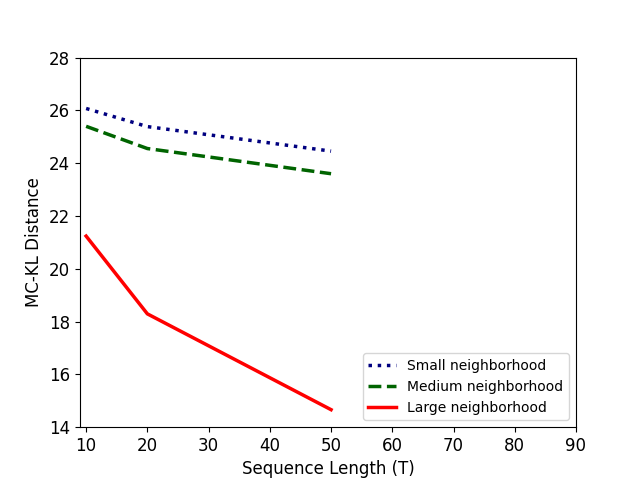
\includegraphics[scale=0.8]{ChapterTwo/KL.png}
	\caption{Monte Carlo approximation of the Kullback-Leibler divergence between the random and reference HMMs with different neighborhood sizes and sequence lengths.}
	\label{fig:sohmmm_dist_neig}      
\end{figure}

\section{SpaMHMM: Sparse Mixture of Hidden Markov Models for Graph Connected Entities}
\label{sec:spamhmm}

\subsection{Overview}

Inspired by the formulation of \eqref{sparse_coding}, we propose to model the generative distribution of the data coming from each of the $K$ nodes of a network as a sparse mixture obtained from a dictionary of generative distributions. Specifically, we shall model the distribution for each node as a sparse mixture over a `large' shared dictionary of HMMs, where each HMM corresponds to an individual atom from the dictionary.
The field knowledge about the similarities between nodes is summarized in an affinity matrix. The objective function of the learning process promotes reusing HMM atoms between similar nodes.
We now formalize these ideas.

\subsection{Model formulation}
\subsubsection{Definition}
\label{sec:definition}
Assume we have a set of nodes $\sY=\{1, \dots, K\}$ connected by an undirected weighted graph $\gG$, expressed by a symmetric matrix $\mG \in \R^{K \times K}$. These nodes thus form a network, in which the weights are assumed to represent degrees of affinity between each pair of nodes (i.e.\ the greater the edge weight, the more the respective nodes \textit{like} to agree). The nodes $\ry$ in the graph produce $D$-dimensional sequences $\rmX = \left(\rvx^{(1)}, \dots,\rvx^{(T)} \right)$, $\rvx^{(t)} \in \R^D$, whose conditional distribution we shall model using a mixture of HMMs:
\begin{equation}
\label{hmm_mix}
p(\rmX \mid \ry) = \sum_{\rz} p(\rz\mid\ry) p(\rmX \mid \rz),
\end{equation}
where $\rz \in \{1, \dots, M\}$ is a latent random variable, being $M$ the size of the mixture. This is a particular realization of \eqref{sparse_coding} where $f$ is the probability density function $p(\rmX \mid \ry)$ and the coefficients $s_m$ correspond to the probabilities $p(\rz = m \mid \ry)$. Here, $p(\rmX \mid \rz)$ is the marginal distribution of observations of a standard first-order homogeneous HMM:
\begin{equation}
\label{hmm}
p(\rmX \mid \rz) = \sum_{\rvh} p(\rh^{(0)}\mid\rz) \prod_t p(\rh^{(t)}\mid\rh^{(t-1)},\rz) p(\rvx^{(t)}\mid\rh^{(t)},\rz),
\end{equation}
where $\rvh = \left(\rh^{(0)}, \dots,\rh^{(T)} \right)$, $\rh^{(t)} \in \{1, \dots, S\}$, is the sequence of hidden states of the HMM, being $S$ the number of hidden states. Note that the factorization in \eqref{hmm_mix} imposes conditional independence between the sequence $\rmX$ and the node $\ry$, given the latent variable $\rz$. This is a key assumption of this model, since this way the distributions for the observations in the nodes in $\sY$ share the same dictionary of HMMs, promoting parameter sharing among the $K$ mixtures.

\subsubsection{Inference}
\label{sec:inference}
Given an observed sequence $\mX$ and its corresponding node $y \in \sY$, the inference problem here consists in finding the likelihood $p(\rmX=\mX \mid \ry=y)$ (from now on, abbreviated as $p(\mX \mid y)$) as defined by  \twoeqrefs{hmm_mix}{hmm}. The marginals $p(\mX\mid\rz)$ of each HMM in the mixture may be computed efficiently, in $O(S^2T)$ time, using the Forward algorithm~\citet{Rabiner1986}. Then, $p(\mX \mid y)$ is obtained by applying \eqref{hmm_mix}, so inference in the overall model is done in at most $O(MS^2T)$ time. As we shall see, however, the mixtures we get after learning will often be sparse (see \Secref{sec:learning}), leading to an even smaller time complexity.

\subsubsection{Learning}
\label{sec:learning}
Given an i.i.d. dataset consisting of $N$ tuples $(\mX_i, y_i)$ of sequences of observations $\mX_i = \left(\vx_i^{(1)}, \dots,\vx_i^{(T_i)} \right)$ and their respective nodes $y_i \in \sY$, the model defined by \twoeqrefs{hmm_mix}{hmm} may be easily trained using the Expectation-Maximization (EM) algorithm \citet{Dempster1977}, (locally) maximizing the usual log-likelihood objective:
\begin{equation}
\label{log_likelihood}
J(\theta) = \sum_{i=1}^N \log p(\mX_i \mid y_i, \theta),
\end{equation}
where $\theta$ represents all model parameters, namely:
\begin{enumerate}
	\item the $M$-dimensional mixture coefficients, $\valpha_k \coloneqq \left(p(\rz=1\mid\ry=k), \dots, p(\rz=M\mid\ry=k)\right)$, for $k = 1,\dots,K$;
	\item the $S$-dimensional initial state probabilities, $\vpi_m \coloneqq \left(p(\rh^{(0)}=1 \mid \rz=m),\dots,p(\rh^{(0)}=S \mid \rz=m)\right)$, for $m = 1,\dots,M$;
	\item the $S \times S$ state transition matrices, $\mA^m$, where $\emA^m_{s,u} \coloneqq p(\rh^{(t)}=u \mid \rh^{(t-1)}=s, \rz=m)$, for $s,u = 1,\dots,S$ and $m = 1,\dots,M$;
	\item the emission probability means, $\vmu_{m,s} \in \mathbb{R}^D$, for $m = 1,\dots,M$ and $s = 1,\dots,S$;
	\item the emission probability diagonal covariance matrices, $\mI \vsigma^2_{m,s}$, where $\vsigma^2_{m,s} \in \mathbb{R}^{D}_{+}$, for $m = 1,\dots,M$ and $s = 1,\dots,S$.
\end{enumerate}

Here, we are assuming that the emission probabilities $p(\rx^{(t)}\mid\rh^{(t)},\rz)$ are Gaussian with diagonal covariances. This introduces almost no loss of generality, since the extension of this work to discrete observations or other types of continuous emission distributions is straightforward.

The procedure to maximize objective~\plaineqref{log_likelihood} using EM is described in \Algref{alg:mhmm}. The update formulas follow from the standard EM procedure and can be obtained by viewing this model as a Bayesian network or by following the derivation detailed in \Secref{sec:proof_em_noreg}. However, the objective \plaineqref{log_likelihood} does not take advantage of the known structure of $\gG$. In order to exploit this information, we introduce a regularization term, maximizing the following objective instead:
\begin{align}
\label{objective}
J_r(\theta) &= \frac{1}{N}\sum_{i=1}^N \log p(\mX_i \mid y_i, \theta) \nonumber\\ 
&\mathbin{\hphantom{=}}{}+ \frac{\reg}{2} \sum_{\substack{j,k=1,\\k\neq j}}^{K} \emG_{j,k} \E_{\rz \sim p(\rz \mid \ry=j, \theta)} [ p(\rz \mid \ry=k, \theta) ] \nonumber\\
&= \frac{1}{N}\sum_{i=1}^N \log p(\mX_i \mid y_i, \theta) + \frac{\reg}{2} \sum_{\substack{j,k=1,\\k\neq j}}^{K} \emG_{j,k} \valpha_j^\top \valpha_k,
\end{align}
where $\reg \geq 0$ controls the relative weight of the two terms in the objective. Note that this regularization term favors nodes connected by edges with large positive weights to have similar mixture coefficients and thus share mixture components. On the other hand, nodes connected by edges with large negative weights will tend to have orthogonal mixture coefficients, being described by disjoint sets of components. These observations agree with our prior assumption that the edge weights express degrees of similarity between each pair of nodes. Proposition \ref{prop_expectations} formalizes these statements and enlightens interesting properties about the expectations $\E_{\rz \sim p(\rz \mid \ry=j, \theta)} [ p(\rz \mid \ry=k, \theta)]$.
\begin{proposition}
	\label{prop_expectations}
	For any integer $M>1$, let $\sP_M$ be the set of all probability distributions over the set $\{1,2\dots,M\}$. We have:
	\begin{enumerate}
		\item $\min_{p,q \in \sP_M} \E_{\rz\sim p} [ q(\rz) ] = 0$; \label{prop_min}
		\item $\argmin_{p,q \in \sP_M} \E_{\rz\sim p} [ q(\rz) ] = \{p,q \in \sP_M \mid \forall \, m \in \{1,\dots,M\}: p(\rz = m)q(\rz = m)=0\}$; \label{prop_argmin}
		\item $\max_{p,q \in \sP_M} \E_{\rz\sim p} [ q(\rz) ] = 1$; \label{prop_max}
		\item $\argmax_{p,q \in \sP_M} \E_{\rz\sim p} [ q(\rz) ] = \{p,q \in \sP_M \mid \exists \, m \in \{1,\dots,M\} : \, p(\rz = m)=q(\rz = m)=1\}$ \label{prop_argmax}.
	\end{enumerate}
\end{proposition}
\begin{proof}
	By the definition of expectation,
	\begin{equation}
	\label{prop_expdef}
	\E_{\rz\sim p} [ q(\rz) ] = \sum_{m=1}^M p(\rz=m) q(\rz=m).
	\end{equation}
	Statements \ref{prop_min} and \ref{prop_argmin} follow immediately from the fact that every term in the right-hand side of \plaineqref{prop_expdef} is non-negative and $M>1$. For the remaining, we rewrite \plaineqref{prop_expdef} as the dot product of two $M$-dimensional vectors $\valpha_p$ and $\valpha_q$, representing the two distributions $p$ and $q$, respectively, and we use the following linear algebra inequalities to build an upper bound for this expectation:
	\begin{equation}
	\label{prop_ineq}
	\E_{\rz\sim p} [ q(\rz) ] = \valpha_p ^\top \valpha_q \leq || \valpha_p ||_2 || \valpha_q ||_2 \leq || \valpha_p ||_1 || \valpha_q ||_1 =1,
	\end{equation}
	where $||\bcdot||_1$ and $||\bcdot||_2$ are the $\normlone$ and $\normltwo$ norms, respectively. Clearly, the equality $\E_{\rz\sim p} [ q(\rz) ] = 1$ holds if $p$ and $q$ are chosen from the set defined in statement \ref{prop_argmax}, where the distributions $p$ and $q$ are the same and they are non-zero for a single assignment of $\rz$. This proves statement \ref{prop_max}. Now, to prove statement \ref{prop_argmax}, it suffices to show that there are no other maximizers. The first inequality in \plaineqref{prop_ineq} is transformed into an equality if and only if $\valpha_p = \valpha_q$, which means $p \equiv q$. The second inequality becomes an equality when the $\normlone$ and $\normltwo$ norms of the vectors coincide, which happens if and only if the vectors have only one non-zero component, concluding the proof.
\end{proof}
Specifically, given two distinct nodes $j, k \in \sY$ , if $\emG_{j,k} > 0$, the regularization term for these nodes is maximum (and equal to $\emG_{j,k}$) when the mixtures for these two nodes are the same and have one single active component (i.e.\ one mixture component whose coefficient is non-zero). On the contrary, if $\emG_{j,k} < 0$, the term is maximized (and equal to zero) when the mixtures for the two nodes do not share any active components. In both cases, though, we conclude from Proposition \ref{prop_expectations} that we are favoring sparse mixtures. We see sparsity as an important feature since it allows the size $M$ of the dictionary of models to be large and therefore expressive without compromising our rational that the observations in a given node are well modeled by a mixture of only a few HMMs. This way, some components will specialize on describing the behavior of some nodes, while others will specialize on different nodes. Moreover, sparse mixtures yield faster inference, more interpretable models and (possibly) less overfitting.
By setting $\reg=0$, we clearly get the initial objective \plaineqref{log_likelihood}, where inter-node correlations are modeled only via parameter sharing. As $\reg \to \infty$, two interesting scenarios may be anticipated. If $\emG_{j,k} > 0, \, \forall j,k \in \sY,$ all nodes will tend do share the same single mixture component, i.e.\ we would be learning one single HMM to describe the whole network. If $\emG_{j,k} < 0, \, \forall j,k \in \sY,$ and $M \geq K$, each node would tend to learn its own HMM model independently from all the others. Again, in both scenarios, the obtained mixtures are sparse.

The objective function~\plaineqref{objective} can still be maximized via EM (see details in \Secref{sec:proof_em_reg}). However, the introduction of the regularization term in the objective makes it impossible to find a closed form solution for the update formula of the mixture coefficients. Thus, in the M-step, we need to resort to gradient ascent to update these parameters. In order to ensure that the gradient ascent iterative steps lead to admissible solutions, we adopt the following reparametrization from \citet{Yang2018}:
\begin{equation}
\label{normalization}
\alpha_{k,m} = \frac{\sigma \left(\beta_{k,m} \right)^2}{\sum_{l=1}^M \sigma \left( \beta_{k,l} \right)^2}, 
\end{equation}
for $k = 1, \dots, K$ and $m = 1, \dots, M$, and where $\sigma(\bcdot)$ is the rectifier linear (ReLU) function. This reparametrization clearly resembles the softmax function, but, contrarily to that one, admits sparse outputs. The squared terms in \eqref{normalization} aim only to make the optimization more stable. The optimization steps for the objective \plaineqref{objective} using this reparametrization are described in \Algref{alg:spamhmm}.

\begin{algorithm}
	\caption{EM algorithm for the mixture without regularization (MHMM).}
	\label{alg:mhmm}
	\begin{algorithmic}
		\State Inputs: The training set, consisting of $N$ tuples $(\mX_i,y_i)$, a set of initial parameters $\theta^{(0)}$ and the number of training iterations $\mathcal{I}$.
		\For{$j = 1, \dots, \mathcal{I}$}
		\State Sufficient statistics:
		\begin{enumerate}
			\item $n_k \coloneqq \sum_i \1_{y_i=k}$, where $\1_\mathrm{(\bcdot)}$ is the indicator function, for $k=1,\dots,K$.
			\item Obtain the mixture posteriors $\eta_{i,m} \coloneqq p(\rz=m|\mX_i, y_i,\theta^{(j-1)})$, for $i=1,\dots,N$ and $m=1,\dots,M$, by computing  $\tilde{\eta}_{i,m} \coloneqq p(\mX_i|\rz=m, \theta^{(j-1)})p(\rz=m|y_i, \theta^{(j-1)})$ and normalizing it.
			\item Obtain the state posteriors $\gamma_{i,m,s}(t) \coloneqq p(\rh^{(t)}=s | \rz=m, \mX_i, \theta^{(j-1)})$ and $\xi_{i,m,s,u}(t) \coloneqq p(\rh^{(t-1)}=s, \rh^{(t)}=u | \rz=m, \mX_i, \theta^{(j-1)})$, for $i=1,\dots,N$, $m=1,\dots,M$ and $s,u=1,\dots,S$, as done in the Baum-Welch algorithm \citet{Baum1972}.
		\end{enumerate}
		\State M-step:
		\begin{enumerate}
			\item $\evalpha_{k,m} = \frac{\sum_i \eta_{i,m} \1_{y_i=k}}{n_k}$, for $k=1,\dots,K$ and $m=1,\dots,M$, obtaining $\valpha_k$.
			\item $\evpi_{m,s} = \frac{\sum_i \eta_{i,m} \gamma_{i,m,s}(0)}{\sum_i \eta_{i,m}}$, for $m=1,\dots,M$ and $s=1,\dots,S$, obtaining $\vpi_{m}$. 
			\item $\emA^m_{s,u} = \frac{\sum_i \eta_{i,m} \sum_{t=1}^{T_i} \xi_{i,m,s,u}(t)}{\sum_i \eta_{i,m} \sum_{t=0}^{T_i-1} \gamma_{i,m,s}(t)}$, for $m=1,\dots,M$ and $s,u=1,\dots,S$, obtaining $\mA^m$.
			\item $\vmu_{m,s} = \frac{\sum_i \eta_{i,m} \sum_{t=1}^{T_i} \gamma_{i,m,s}(t) \vx_i^{(t)}} {\sum_i \eta_{i,m} \sum_{t=1}^{T_i} \gamma_{i,m,s}(t)}$, for $m=1,\dots,M$ and $s=1,\dots,S$.
			\item $\vsigma^2_{m,s} = \frac{\sum_i \eta_{i,m} \sum_{t=1}^{T_i} \gamma_{i,m,s}(t) \left(\vx_i^{(t)} - \boldsymbol{\mu}^m_s\right)^2} {\sum_i \eta_{i,m} \sum_{t=1}^{T_i} \gamma_{i,m,s}(t)}$, for $m=1,\dots,M$ and $s=1,\dots,S$.
			\item $\theta^{(j)} = \bigcup_{k,m,s} \left\lbrace \boldsymbol{\alpha}_k, \vpi_{m}, \mA^m, \vmu_{m,s}, \vsigma^2_{m,s} \right\rbrace$.
		\end{enumerate}
		\EndFor  
	\end{algorithmic}
\end{algorithm}

\begin{algorithm}
	\caption{EM algorithm for the mixture with regularization (SpaMHMM).}
	\label{alg:spamhmm}
	\begin{algorithmic}
		\State Inputs: The training set, consisting of $N$ tuples $(\mX_i,y_i)$, the matrix $\mG$ describing the graph $\gG$, the regularization hyperparameter $\reg$, a set of initial parameters $\theta^{(0)}$, the number of training iterations $\mathcal{I}$, the number of gradient ascent iterations $\mathcal{J}$ to perform on each M-step, the learning rate $\rho$ for the gradient ascent.
		\For{$j=1,\dots,\mathcal{I}$}
		\State Sufficient statistics: same as in \Algref{alg:mhmm}.
		\State M-step:
		\For{$l=1,\dots,\mathcal{J}$}
		\begin{enumerate}
			\item $\psi_{k,m} \coloneqq \frac{1}{N}\sum_i (\eta_{i,m} - \alpha_{k,m}) \1_{y_i=k}$, for $k=1,\dots,K$ and $m=1,\dots,M$.
			\item $\omega_{k,m} \coloneqq \alpha_{k,m} \sum_{j \neq k} \emG_{j,k}\left(\alpha_{j,m} - \valpha_j \transp \valpha_k \right)$, for $k=1,\dots,K$ and $m=1,\dots,M$.
			\item $\delta_{k,m} \coloneqq \1_{\beta_{k,m} > 0} \frac{2\sigma'(\beta_{k,m})}{\sigma(\beta_{k,m})}\left(\psi_{k,m} + \reg \omega_{k,m}\right)$, where $\sigma'(\cdot)$ is the derivative of $\sigma(\cdot)$, for $k=1,\dots,K$ and $m=1,\dots,M$. 
			\item $\beta_{k,m} \leftarrow \beta_{k,m} + \rho \delta_{k,m}$, for $k=1,\dots,K$ and $m=1,\dots,M$.
			\item Use \eqref{normalization} to obtain $\alpha_{k,m}$, for $k=1,\dots,K$ and $m=1,\dots,M$.
		\end{enumerate}
		\EndFor
		\State Do steps 2) -- 6) in the M-step of \Algref{alg:mhmm}. 
		\EndFor
	\end{algorithmic}
\end{algorithm}

\section{Experimental Evaluation}
\label{sec:experiments}
The model was developed on top of the library hmmlearn~\citet{hmmlearn} for Python, which implements inference and unsupervised learning for the standard HMM using a wide variety of emission distributions. Both learning and inference use the hmmlearn API, with the appropriate adjustments for our models. For reproducibility purposes, we make our source code, pre-trained models and the datasets publicly available \footnote{\url{https://github.com/dpernes/spamhmm}}.

We evaluate four different models in our experiments: a model consisting of a single HMM (denoted as 1-HMM) trained on sequences from all graph nodes; a model consisting of $K$ HMMs trained independently (denoted as K-HMM), one for each graph node; a mixture of HMMs (denoted as MHMM) as defined in this work (\twoeqrefs{hmm_mix}{hmm}), trained to maximize the usual log-likelihood objective~\plaineqref{log_likelihood}; a mixture of HMMs (denoted as SpaMHMM) as the previous one, trained to maximize our regularized objective~\plaineqref{objective}.

Models 1-HMM, K-HMM and MHMM will be our baselines. We shall compare the performance of these models with that of SpaMHMM and, for the case of MHMM, we shall also verify if SpaMHMM actually produces sparser mixtures in general, as argued in \Secref{sec:learning}. In order to ensure a fair comparison, we train models with approximately the same number of possible state transitions. Hence, given an MHMM or SpaMHMM with $M$ mixture components and $S$ states per component, we train a 1-HMM with $\approx S\sqrt[]{M}$ states and a K-HMM with $\approx S\sqrt[]{M/K}$ states per HMM. We initialize the mixture coefficients in MHMM and SpaMHMM randomly, while the state transition matrices and the initial state probabilities are initialized uniformly. Means are initialized using $k$-means, with $k$ equal to the number of hidden states in the HMM, and covariances are initialized with the diagonal of the training data covariance. Models 1-HMM and K-HMM are trained using the Baum-Welch algorithm, MHMM is trained using \Algref{alg:mhmm} and SpaMHMM is trained using \Algref{alg:spamhmm}. However, we opted to use Adam \citet{Kingma2014} instead of \textit{vanilla} gradient ascent in the inner loop of \Algref{alg:spamhmm}, since its per-parameter learning rate proved to be beneficial for faster convergence.

\subsection{Anomaly detection in Wi-Fi networks}
\label{sec:wi_fi}
A typical Wi-Fi network infrastructure is constituted by $K$ access points (APs) distributed in a given space. The network users may alternate between these APs seamlessly, usually connecting to the closest one. There is a wide variety of anomalies that may happen during the operation of such network and their automatic detection is, therefore, of great importance for future mitigation plans. Some anomalous behaviors are: overloaded APs, failed or crashed APs, persistent radio frequency interference between adjacent APs, authentication failures, etc. However, obtaining reliable ground truth annotation of these anomalies in entire wireless networks is costly and time consuming. Under these circumstances, using data obtained through realistic network simulations is a common practice. 

In order to evaluate our model in the aforementioned scenario, we have followed the procedure of \citet{Anisa2017}, performing extensive network simulations in a typical Wi-Fi network setup (IEEE 802.11 WLANg 2.4 GHz in infrastructure mode) using OMNeT++~\citet{omnetpp} and INET~\citet{inet} simulators. Our network consists of 10 APs and 100 users accessing it. The pairwise distances between APs are known and fixed. Each sequence contains information about the traffic in a given AP during 10 consecutive hours and is divided in time slots of 15 minutes without overlap. Thus, every sequence has the same length, which is equal to 40 samples (time slots). Each sample contains the following 7 features: the number of unique users connected to the AP, the number of sessions within the AP, the total duration (in seconds) of association time of all current users, the number of octets transmitted and received in the AP and the number of packets transmitted and received in the AP. Anomalies typically occur for a limited amount of time within the whole sequence. However, in this experiment, we label a sequence as ``anomalous'' if there is at least one anomaly period in the sequence and we label it as ``normal'' otherwise. One of the simulations includes normal data only, while the remaining include both normal and anomalous sequences. In order to avoid contamination of normal data with anomalies that may occur simultaneously in other APs, we used the data of the normal simulation for training (150 sequences) and the remaining data for testing (378 normal and 42 anomalous sequences). 

In a Wi-Fi network, as users move in the covered area, they disconnect from one AP and they immediately connect to another in the vicinity. As such, the traffic in adjacent APs may be expected to be similar. Following this idea, the weight $\emG_{j,k}$, associated with the edge connecting nodes $j$ and $k$ in graph $\gG$, was set to the inverse distance between APs $j$ and $k$ and normalized so that $\max_{j,k} G_{j,k}=1$. As in \citet{Anisa2017}, sequences were preprocessed by subtracting the mean and dividing by the standard deviation and applying PCA, reducing the number of features to 3. For MHMM, we did 3-fold cross validation of the number of mixture components $M$ and hidden states per component $S$. We ended up using $M=15$ and $S=10$. We then used the same values of $M$ and $S$ for SpaMHMM and we did 3-fold cross validation for the regularization hyperparameter $\reg$ in the range $[10^{-4}, 1]$. The value $\reg=10^{-1}$ was chosen. We also cross-validated the number of hidden states in 1-HMM and K-HMM around the values indicated in \Secref{sec:experiments}. Every model was trained for 100 EM iterations or until the loss plateaus. For SpaMHMM, we did 100 iterations of the inner loop on each M-step, using a learning rate $\rho=10^{-3}$. We repeat training 10 times for each model, starting from different random initializations, in order to reduce the likelihood of erroneous results due to local minima trapping.

Models were evaluated by computing the average log-likelihood per sample on normal and anomalous test data, plotting the receiver operating characteristic (ROC) curves and computing the respective areas under the curves (AUCs). The small standard deviations in \Tableref{tbl:wifi_results} attest the robustness of the adopted initialization scheme and learning algorithms. \Figref{fig:roc} shows that the ROC curves for MHMM and SpaMHMM are very similar and that these models clearly outperform 1-HMM and K-HMM. This is confirmed by the AUC and log-likelihood results in \Tableref{tbl:wifi_results}. Although K-HMM achieved the best (lowest) average log-likelihood on anomalous data, this result is not relevant, since it also achieved the worst (lowest) average log-likelihood on normal data. This is in fact the model with the worst performance, as shown by its ROC and respective AUC.

The bad performance of K-HMM likely results mostly from the small amount of data that each of the $K$ models is trained with: in K-HMM, each HMM is trained with the data from the graph node (AP) that it is assigned to. The low log-likelihood value of the normal test data in this model confirms that the model does not generalize well to the test data and is probably highly biased towards the training data distribution. On the other hand, in 1-HMM there is a single HMM that is trained with the whole training set. However, the same HMM needs to capture the distribution of the data coming from all APs. Since each AP has its own typical usage profile, these data distributions are different and one single HMM may not be sufficiently expressive to learn all of them correctly. MHMM and SpaMHMM combine the advantages and avoid the disadvantages of both previous models. Clearly, since the mixtures for each node share the same dictionary of HMMs, every model in the mixture is trained with sequences from all graph nodes, at least in the first few training iterations. Thus, at this stage, the models may capture behaviors that are shared by all APs. As mixtures become sparser during training, some components in the dictionary may specialize on the distribution of a few APs. This avoids the problem observed in 1-HMM, which is unaware of the AP where a sequence comes from. We would also expect SpaMHMM to be sparser and have better performance than MHMM, but only the former supposition was true (see \Figref{fig:sparsity}). The absence of performance gains in SpaMHMM might be explained from the fact that this dataset consists of simulated data, where users are static (i.e.\ they do not swap between APs unless the AP where they are connected stops working) and so the assumption that closer APs have similar distributions does not bring any advantage.

\begin{figure}
	\centering
	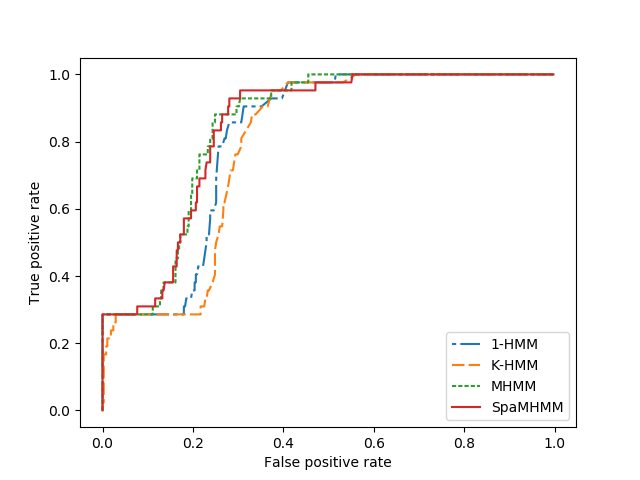
\includegraphics[width=0.8\linewidth]{ChapterTwo/roc.png}
	\caption{ROC curves for each model on the Wi-Fi dataset, for one of the 10 runs.}
	\label{fig:roc}
\end{figure}

\begin{table}
	\centering
	\begin{tabular}{l|r|r r}
		\multicolumn{1}{c}{} & \multicolumn{1}{c}{} & \multicolumn{2}{c}{Average log-likelihood} \\
		& \multicolumn{1}{c|}{AUC} & Normal data & Anomalous data \\
		\hline
		1-HMM & $0.806~(\pm 0.01)$ & $-6.36~(\pm 0.66)$ & $-129.40~(\pm 22.22)$ \\
		K-HMM & $0.776~(\pm 0.01)$ & $-22.09~(\pm 1.12)$ & $\mathbf{-130.36}~(\pm 26.30)$ \\
		MHMM & $\mathbf{0.830}~(\pm 0.01)$ & $-3.31~(\pm 0.21)$ & $-10.99~(\pm 1.10)$ \\
		SpaMHMM & $0.829~(\pm 0.01)$ & $\mathbf{-3.26}~(\pm 0.12)$ & $-11.29~(\pm 1.39)$ \\
	\end{tabular}
	\caption{AUC and average log-likelihood per sample for each model in the Wi-Fi dataset averaged over 10 training runs. Standard deviations are in brackets. Best results are in bold.}
	\label{tbl:wifi_results}
\end{table}

\subsection{Human motion forecasting}
\label{sec:h36m}
The human body is constituted by several interdependent parts, which interact as a whole producing sensible global motion patterns. These patterns may correspond to multiple activities like walking, eating, etc. Here, we use our model to make short-time prediction of sequences of human joint positions, represented as motion capture (mocap) data. The current state of the art methodologies use architectures based on deep recurrent neural networks (RNNs), achieving remarkable results both in short-time prediction \citet{Fragkiadaki2015, Martinez2017} and in long-term motion generation \citet{Jain2016, Pavllo2018}.

Our experiments were conducted on the Human3.6M dataset from \citet{Ionescu2011, Ionescu2014}, which consists of mocap data from 7 subjects performing 15 distinct actions. In this experiment, we have considered only 4 of those actions, namely ``walking'', ``eating'', ``smoking'' and ``discussion''. There, the human skeleton is represented with 32 joints whose position is recorded at 50 Hz. We build our 32x32-dimensional symmetric matrix $\mG$ representing the graph $\gG$ in the following sensible manner: $G_{j,k}=1$, if there is an actual skeleton connection between joints $j$ and $k$ (e.g.\  the elbow joint is connected to the wrist joint by the forearm); $G_{j,k}=1$, if joints $j$ and $k$ are symmetric (e.g.\  left and right elbows); $G_{j,k}=0$, otherwise.

\subsubsection{Forecasting}

We reproduced as much as possible the experimental setup followed in \citet{Fragkiadaki2015}. Specifically, we down-sampled the data by a factor of 2 and transformed the raw 3-D angles into an exponential map representation. We removed joints with constant exponential map, yielding a dataset with 22 distinct joints, and pruned our matrix $\mG$ accordingly. Training was performed using data from 6 subjects, leaving one subject (denoted in the dataset by ``S5'') for testing. We did 3-fold cross-validation on the training data of the action ``walking'' to find the optimal number of mixture components $M$ and hidden states $S$ for the baseline mixture MHMM. Unsurprisingly, since this model can hardly overfit in such a complex task, we ended up with $M=18$ and $S=12$, which were the largest values in the ranges we defined. Larger values are likely to improve the results, but the training time would become too large to be practical. For SpaMHMM, we used these same values of $M$ and $S$ and we did 3-fold cross validation on the training data of the action ``walking'' to fine-tune the value of $\reg$ in the range $[10^{-4}, 1]$. We ended up using $\reg=0.05$. The number of hidden states in 1-HMM was set to 51 and in K-HMM it was set to 11 hidden states per HMM. The same values were then used to train the models for the remaining actions. Every model was trained for 100 iterations of EM  or until the loss plateaus. For SpaMHMM, we did 100 iterations of the inner loop on each M-step, using a learning rate $\rho=10^{-2}$.

In order to generate predictions for a joint (node) $y$ starting from a given prefix sequence $\mX_{\text{pref}}$, we compute the posterior distribution $p(\rmX | \mX_{\text{pref}}, y)$ (see details in \Secref{sec:posterior_proof}) and we sample sequences from that posterior. Our evaluation method and metric again followed \citet{Fragkiadaki2015}. We fed our model with 8 prefix subsequences with 50 frames each (corresponding to 2 seconds) for each joint from the test subject and we predicted the following 10 frames (corresponding to 400 miliseconds). Each prediction was built by sampling 100 sequences from the posterior and averaging. We then computed the average mean angle error for the 8 sequences at different time horizons. 

Results are in \Tableref{tbl:h36m_results}. Among our models (1-HMM, K-HMM, MHMM and SpaMHMM), SpaMHMM outperformed the remaining in all actions except ``eating''. For this action in particular, MHMM was slightly better than SpaMHMM, probably due to the lack of symmetry between the right and left sides of the body, which was one of the prior assumptions that we have used to build the graph $\gG$. ``Smoking'' and ``discussion'' activities may also be highly non-symmetric, but results in our and others' models show that these activities are generally harder to predict than ``walking'' and ``eating'. Thus, here, the skeleton structure information encoded in $\gG$ behaves as a useful prior for SpaMHMM, guiding it towards better solutions than MHMM. The worse results for 1-HMM and K-HMM likely result from the same limitations that we have pointed out in \Secref{sec:wi_fi}: each component in K-HMM is inherently trained with less data than the remaining models, while 1-HMM does not make distinction between different graph nodes. Extending the discussion to the state of the art solutions for this problem, we note that SpaMHMM compares favorably with ERD, LSTM-3LR and SRNN, which are all RNN-based architectures. Moreover, ERD and LSTM-3LR were designed specifically for this task, which is not the case for SpaMHMM. This is also true for GRU supervised and QuaterNet, which clearly outperform all remaining models, including ours. This is unsurprising, since RNNs are capable of modeling more complex dynamics than HMMs, due to their intrinsic non-linearity and continuous state representation. This also allows their usage for long-term motion generation, in which HMMs do not behave well due their linear dynamics and lack of long-term memory. However, unlike GRU supervised and QuaterNet, SpaMHMM  models the probability distribution of the data directly, allowing its application in domains like novelty detection. Regarding sparsity, the experiments confirm that the SpaMHMM mixture coefficients are actually sparser than those of MHMM, as shown in \Figref{fig:sparsity}.

\begin{table*}
	\resizebox{\textwidth}{!}{
		\begin{tabular}{l|c c c c| c c c c| c c c c | c c c c}
			\multicolumn{1}{c}{} & \multicolumn{4}{c}{Walking} & \multicolumn{4}{c}{Eating} & \multicolumn{4}{c}{Smoking} & \multicolumn{4}{c}{Discussion} \\
			miliseconds & 80 & 160 & 320 & 400 & 80 & 160 & 320 & 400 & 80 & 160 & 320 & 400 & 80 & 160 & 320 & 400 \\
			\hline
			1-HMM & 0.91 & 1.04 & 1.22 & 1.31 & 1.00 & 1.08 & 1.15 & 1.21 & 1.45 & 1.55 & 1.70 & 1.75 & 1.19 & 1.42 & 1.55 & 1.56 \\
			K-HMM & 1.29 & 1.33 & 1.34 & 1.38 & 1.16 & 1.22 & 1.28 & 1.34 & 1.70 & 1.77 & 1.90 & 1.95 & 1.47 & 1.61 & 1.68 & 1.63 \\
			MHMM & \textbf{0.78} & \textbf{0.93} & 1.13 & 1.21 & \textbf{0.77} & \textbf{0.87} & \textbf{0.98} & \textbf{1.06} & 1.44 & 1.53 & 1.69 & 1.77 & 1.14 & 1.36 & 1.52 & 1.54 \\
			SpaMHMM & 0.80 & \textbf{0.93} & \textbf{1.11} & \textbf{1.18} & 0.81 & 0.90 & 0.99 & \textbf{1.06} & \textbf{1.29} & \textbf{1.39} & \textbf{1.61} & \textbf{1.67} & \textbf{1.09} & \textbf{1.30} & \textbf{1.44} & \textbf{1.49} \\
			\hline
			ERD \citet{Fragkiadaki2015} & 0.93 & 1.18 & 1.59 & 1.78 & 1.27 & 1.45 & 1.66 & 1.80 & 1.66 & 1.95 & 2.35 & 2.42 & 2.27 & 2.47 & 2.68 & 2.76 \\
			LSTM-3LR \citet{Fragkiadaki2015} & 0.77 & 1.00 & 1.29 & 1.47 & 0.89 & 1.09 & 1.35 & 1.46 & 1.34 & 1.65 & 2.04 & 2.16 & 1.88 & 2.12 & 2.25 & 2.23 \\
			SRNN \citet{Jain2016} & 0.81 & 0.94 & 1.16 & 1.30 & 0.97 & 1.14 & 1.35 & 1.46 & 1.45 & 1.68 & 1.94 & 2.08 & 1.22 & 1.49 & 1.83 & 1.93 \\
			GRU sup. \citet{Martinez2017} & 0.28 & 0.49 & 0.72 & 0.81 & 0.23 & 0.39 & 0.62 & 0.76 & 0.33 & 0.61 & 1.05 & 1.15 & 0.31 & 0.68 & 1.01 & 1.09 \\
			QuaterNet \citet{Pavllo2018} & \underline{0.21} & \underline{0.34} & \underline{0.56} & \underline{0.62} & \underline{0.20} & \underline{0.35} & \underline{0.58} & \underline{0.70} & \underline{0.25} & \underline{0.47} & \underline{0.93} & \underline{0.90} & \underline{0.26} & \underline{0.60} & \underline{0.85} & \underline{0.93}
	\end{tabular}}
	\caption{Mean angle error for short-term motion prediction on Human3.6M for different actions and time horizons. The results for ERD, LSTM-3LR, SRNN, GRU supervised and QuaterNet were extracted from \citet{Pavllo2018}. Best results among our models are in bold, best overall results are underlined.}
	\label{tbl:h36m_results}
\end{table*}

\begin{figure}
	\centering
	\begin{minipage}{.3\textwidth}
		\centering
		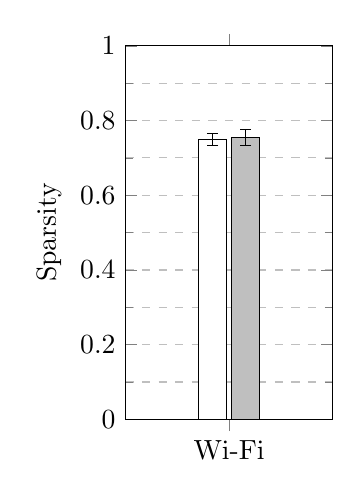
\begin{tikzpicture}
			\begin{axis}[
			ybar,
			bar width=10pt,
			width=120pt,
			height=180pt,
			xmin=Wi-Fi, xmax=Wi-Fi,
			symbolic x coords={Wi-Fi},
			xtick=data,
			ylabel=Sparsity,
			ymin=0, ymax=1,
			ymajorgrids,
			major grid style={dashed},
			yminorgrids,
			minor grid style={dashed},
			minor tick num=1,
			]
			\addplot[fill=white, error bars/.cd, y dir=both, y explicit] 
			coordinates {(Wi-Fi, 0.749) +- (Wi-Fi, 0.017)};
			\addplot[fill=lightgray, error bars/.cd, y dir=both, y explicit] 
			coordinates {(Wi-Fi, 0.755) +- (Wi-Fi, 0.022)};
			\legend{}
			\end{axis}
		\end{tikzpicture}
	\end{minipage}%
	\begin{minipage}{.7\textwidth}
		\centering
		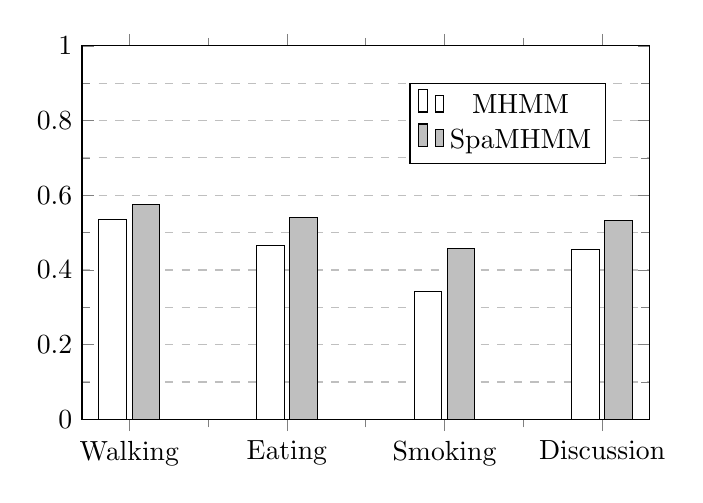
\begin{tikzpicture}
			\begin{axis}[
			ybar,
			bar width=10pt,
			width=250pt,
			height=180pt,
			symbolic x coords={Walking,Eating,Smoking,Discussion},
			xtick=data,
			ymin=0, ymax=1,
			ymajorgrids,
			major grid style={dashed},
			yminorgrids,
			minor grid style={dashed},
			minor tick num=1,
			legend style={at={(0.75,0.9)},
				anchor=north,legend columns=1},
			]
			\addplot[fill=white] 
			coordinates {(Walking,0.535) (Eating,0.465) (Smoking,0.343) (Discussion,0.455)};
			\addplot[fill=lightgray] 
			coordinates {(Walking,0.576) (Eating,0.540) (Smoking,0.457) (Discussion,0.533)};
			\legend{MHMM,SpaMHMM}
			\end{axis}
		\end{tikzpicture}
	\end{minipage} 
	\caption{Relative sparsity (number of coefficients equal to zero / total number of coefficients) of the obtained MHMM and SpaMHMM models on the Wi-Fi dataset (left) and on the Human3.6M dataset for different actions (right). For the Wi-Fi dataset, the average value over the 10 training runs is shown together with the standard deviation. Both models for the Wi-Fi dataset have 150 coefficients. All models for the Human3.6M dataset have 396 coefficients.}
	\label{fig:sparsity}
\end{figure}

\subsubsection{Joint cluster analysis}
\label{sec:spamhmm_cluster}
We may roughly divide the human body in four distinct parts: upper body (head, neck and shoulders), arms, torso and legs. Joints that belong to the same part naturally tend to have coherent motion, so we would expect them to be described by more or less the same components in our mixture models (MHMM and SpaMHMM). Since SpaMHMM is trained to exploit the known skeleton structure, this effect should be even more apparent in SpaMHMM than in MHMM. In order to confirm this conjecture, we have trained MHMM and SpaMHMM for the action ``walking'' using four mixture components only, i.e.\ $M=4$, and we have looked for the most likely component (cluster) for each joint:
\begin{equation}
C_k = \argmax_{m \in \{1,\dots,M\}} p(\rz=m | \ry=k) = \argmax_{m \in \{1,\dots,M\}} \alpha_{k,m},
\end{equation}
where $C_k$ is, therefore, the cluster assigned to joint $k$. The results are in \Figref{fig:clusters}. From there we can see that MHMM somehow succeeds on dividing the body in two main parts, by assigning the joints in the torso and in the upper body mostly to the red/'+' cluster, while those in the hips, legs and feet are almost all assigned to the green/`\SmallTriangleUp' cluster. Besides, we see that in the vast majority of the cases, symmetric joints are assigned to the same cluster. These observations confirm that we have chosen the graph $\gG$ for this problem in an appropriate manner. However, some assignments are unnatural: e.g.\  one of the joints in the left foot is assigned to the red/`+' cluster and the blue/`$\circ$' cluster is assigned to one single joint, in the left forearm. We also observe that the distribution of joints per clusters is highly uneven, being the green/`\SmallTriangleUp' cluster the most represented by far. SpaMHMM, on the other hand, succeeds on dividing the body in four meaningful regions: upper body and upper spine in the green/`\SmallTriangleUp' cluster; arms in the blue/`$\circ$' cluster; lower spine and hips in the orange/`x' cluster; legs and feet in the red/`+' cluster. Note that the graph $\gG$ used to regularize SpaMHMM does not include any information about the body part that a joint belongs to, but only about the joints that connect to it and that are symmetric to it. Nevertheless, the model is capable of using this information together with the training data in order to divide the skeleton in an intuitive and natural way. Moreover, the distribution of joints per cluster is much more even in this case, what may also help to explain why SpaMHMM outperforms MHMM: by splitting the joints more or less evenly by the different HMMs in the mixture, none of the HMM components is forced to learn too many motion patterns. In MHMM, we see that the green/`+' component, for instance, is the most responsible to model the motion of almost all joints in the legs and hips and also some joints in the arms and the red/`+' component is the prevalent on the prediction of the motion patterns of the neck and left foot, which are presumably very different.

\begin{figure*}
	\centering
	\begin{minipage}{.5\textwidth}
		\centering
		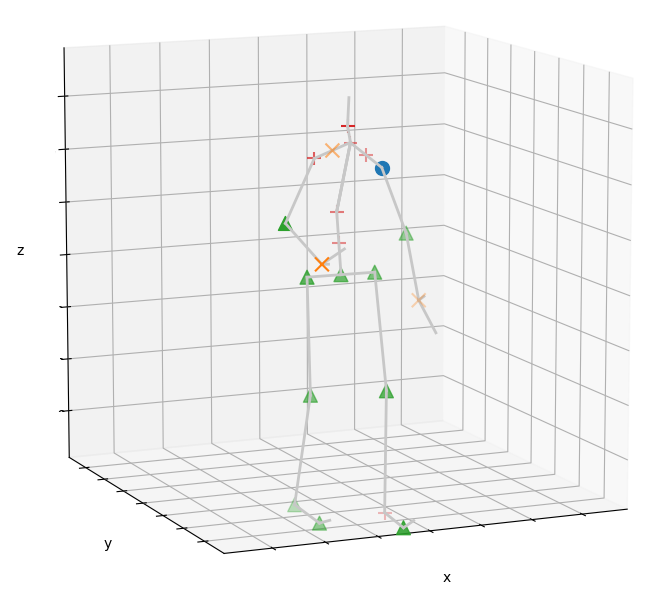
\includegraphics[width=0.8\linewidth]{ChapterTwo/mhmm_clusters}
	\end{minipage}%
	\begin{minipage}{.5\textwidth}
		\centering
		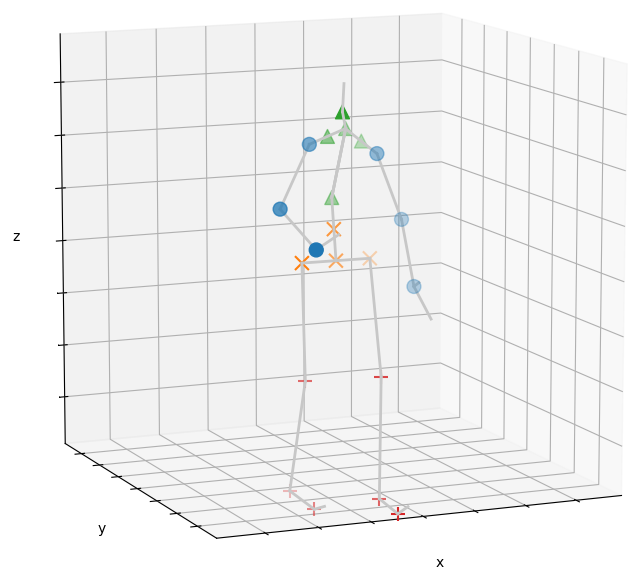
\includegraphics[width=0.8\linewidth]{ChapterTwo/spamhmm_clusters}
	\end{minipage}
	\caption{Assignments of joints to clusters in MHMM (left) and SpaMHMM (right). The different colors (blue, green, orange, red) and the respective symbols (`$\circ$', `\SmallTriangleUp', `x', `+') on each joint represent the cluster that the joint was assigned to. on each joint represent the cluster that the joint was assigned to.}
	\label{fig:clusters}
\end{figure*}
